% coding:utf-8

%----------------------------------------
%FOSAPHY, a LaTeX-Code for a summary of basic physics
%Copyright (C) 2013, Daniel Winz, Ervin Mazlagic

%This program is free software; you can redistribute it and/or
%modify it under the terms of the GNU General Public License
%as published by the Free Software Foundation; either version 2
%of the License, or (at your option) any later version.

%This program is distributed in the hope that it will be useful,
%but WITHOUT ANY WARRANTY; without even the implied warranty of
%MERCHANTABILITY or FITNESS FOR A PARTICULAR PURPOSE.  See the
%GNU General Public License for more details.
%----------------------------------------

\chapter{Wärme}

\newpage
\section{Begriffe}
\begin{table}[h!]
\rowcolors{1}{lgray}{white}
\renewcommand{\arraystretch}{1.5}
\begin{tabular}{p{0.1\textwidth} l c}
$n$		
	& Stoffmenge 		
	& $[mol]$ \\
$N$		
	& Anzahl Teilchen 	
	& - \\
$m$		
	& Masse 		
	& $[kg]$ \\
$m_{mol}$	
	& Molare Masse (siehe Periodensystem, S. \pageref{fig:persys})	
	& $\left[\frac{g}{mol}\right]$ \\
$T$		
	& Tempteratur in Kelvin  ($T = T_{^\circ C} + 273.15 ^\circ C$) 
	& $[K]$ \\
$N_A$	
	& Avogadrozahl ($6.022~141~3 \cdot 10^{23} \frac{1}{mol}$) 
	& - \\
$k_B$		
	& Boltzmannkonstante ($1.380~648~8 \cdot 10^{-23}$)
	& $\left[\frac{J}{K}\right]$ \\ 
$R$	
	& Gaskonstante ($8.314'462'1$)
	& $\left[\frac{J}{mol \cdot K}\right]$
\end{tabular}
\end{table}

\newpage

\begin{comment}
\section{Begriffe}
\[ \begin{array}{@{}ll} 
n:      & \text{Stoffmenge $[mol]$} \\
N:      & \text{Anzahl Teilchen} \\
m:      & \text{Masse} \\
m_{mol}:& \text{Molare Masse 
          (Siehe Periodensystem auf Seite \pageref{fig:persys})} 
          \left\lbrack\frac{g}{mol}\right\rbrack \\
T:      & \text{Tempteratur in $K$ } 
            (T = T_{^\circ C} + 273.15 ^\circ C) \\
N_A:    & \text{Avogadrozahl }
            (6.022~141~3 \cdot 10^{23} \frac{1}{mol}) \\
k_B:    & \text{Boltzmannkonstante } 
            (1.380~648~8 \cdot 10^{-23} \frac{J}{K} ) \\
R:      & \text{Gaskonstante } 
            (8.314~462~1 \frac{J}{mol \cdot K}) \\
\end{array} \]
\end{comment}

\section{Berechnungen zu molaren Grössen}
\[ \boxed{n = \frac{N}{N_A} = \frac{m}{m_{mol}}} \]
Molare Masse von Gasgemischen: 
\[ \boxed{m_{mol_{gem}} = m_{mol_{a}} \cdot \text{Anteil}_a 
+ m_{mol_{b}} \cdot \text{Anteil}_b + \dots} \]
Molare Masse von Molekülen: 
\[ \boxed{m_{kül} = x_1 \cdot m_{mol_a} + x_2 \cdot m_{mol_b} + \dots } 
\qquad x_1, x_2: \text{Anzahl Atome} \]

\section{Gasgleichung}
\[ \boxed{\frac{p \cdot V}{T \cdot n} = const} \]
\[ \boxed{p \cdot V = N \cdot k_B \cdot T 
= n \cdot R \cdot T 
= \frac{N}{N_A} \cdot R \cdot T 
= \frac{m}{m_{mol}} \cdot R \cdot T } \]

\section{Spezifische Wärmekapazität}
\[ \boxed{Q = m \cdot c \cdot \Delta T} \]
\[ \boxed{dQ = m \cdot c \cdot d T} \]
\[ \boxed{c_{(m)} = \frac{1}{m} \frac{dQ}{d T} \qquad \text{c pro Masse}} \]
\[ \boxed{c_{(n)} = \frac{1}{n} \frac{dQ}{d T} \qquad \text{c pro Mol}} \]

\subsection{Spezifische Wärmekapazität von Gasen}
konstantes Gasvolumen
\[ \boxed{C_{(n)V} = C_{V} = \frac{\#FG}{2}R} \]
\begin{tabular}{lcc}
                                      & \#FG     & $C_V$ \\
Ideale Gase: ($Ar$, $Ne$, $He$, ...)  & $3$      & $\nicefrac{3}{2} R$ \\
zwei-atomige: ($O_2$, $N_2$, CO, ...) & $\sim 5$ & $\nicefrac{5}{2} R$ 
\end{tabular}

\subsection{Spezifische Wärme $C_p$ des idealen Gas}
\[ \boxed{C_p = C_v + R} \]
\[ \boxed{\gamma \equiv \frac{C_p}{C_v} = \frac{C_v + R}{C_v}} \]
\[ \gamma = 1.67 \qquad \text{1 atomiges Gas} \]
\[ \gamma = 1.40 \qquad \text{2 atomiges Gas} \]

\section{Volumenarbeit eines Gases}
\[ \boxed{W = -\int_{V_1}^{V_2} p \cdot dV = - p \cdot (V_2 - V_1)} \]

\section{Innere Energie des idealen Gas}
\[ \boxed{U(T) = n \cdot \frac{\#FG}{2} \cdot R \cdot T = n \cdot C_v \cdot T} \]

\section{Zustandsänderungen des idealen Gas}
\[  \begin{array}{ll} 
\Delta p: & \text{Druckänderung} \\
\Delta Q: & \text{Wärmeänderung} \\
\Delta T: & \text{Temperaturänderung} \\
\Delta U: & \text{Änderung der inneren Energie} \\
\Delta V: & \text{Volumenänderung} \\
\Delta W: & \text{Arbeit} \\
\end{array} \]

\subsubsection{isochorer Prozess}
Keine Volumenänderung
\[ \boxed{\Delta V = 0} \qquad \boxed{\Delta W = 0} \]
\[ \boxed{\Delta Q = n \cdot C_v \cdot (T_2 - T_1) = \Delta U} \]

\subsubsection{isobarer Prozess}
Keine Druckänderung
\[ \boxed{\Delta p = 0} \]
\[ \boxed{\Delta U = n \cdot C_v \cdot (T_2 - T_1)} \]
\[ \boxed{\Delta W = - p \cdot (V_2 - V_1) = - n \cdot R \cdot (T_2 - T_1)} \]
\[ \boxed{\Delta Q = n \cdot C_p \cdot (T_2 - T_1)} \]

\subsubsection{isothermer Prozess}
Keine Temperaturänderung
\[ \boxed{\Delta T = 0} \qquad \boxed{\Delta U = 0} \]
\[ \boxed{\Delta W = \int_{V_1}^{V_2} - p dV = - n \cdot R \cdot T \cdot 
\ln\left(\frac{V_2}{V_1}\right) = - \Delta Q} \]

\subsubsection{adiabatischer Prozess}
kein Wärmeaustausch
\[ \boxed{\Delta Q = 0} \]
\[ \boxed{\Delta U = n \cdot C_v \cdot (T_2 - T_1) = \Delta W
= \frac{p_2 \cdot V_2 - p_1 \cdot V_1}{\gamma - 1}} \]
\[ \boxed{T_1 \cdot {V_1}^{(\gamma - 1)} = T_2 \cdot {V_2}^{(\gamma - 1)}} \]
\[ \boxed{p_1 \cdot {V_1}^{\gamma} = p_2 \cdot {V_2}^{\gamma}} \]
\[ \boxed{T_1 \cdot {p_1}^{\left(\frac{1 - \gamma}{\gamma}\right)} 
= T_2 \cdot {p_2}^{\left(\frac{1 - \gamma}{\gamma}\right)}} \]

\section{Druck}
\[ \boxed{p = \frac{F}{A} 
= m_{mol} \cdot {\langle v_x\rangle}^2 \cdot \frac{N}{V}} \]

\section{Barometrische Höhenformel}
Konstante Temperatur
\[ \boxed{p(y) 
= p_0 \cdot e^{- \frac{m_{mol} \cdot g}{R \cdot T} \cdot y} 
= p_0 \cdot e^{- \frac{y}{H}}}\]
\[ \boxed{H = \frac{R \cdot T}{m_{mol} \cdot g} 
\qquad \text{Charakteristische Höhe}} \]
Veränderliche Temperatur
\[ \boxed{p(y) = p_0 \cdot \left(1 - \frac{b}{a} \cdot y\right)^
{\frac{m_{mol} \cdot g}{R \cdot b}} 
= p_0 \cdot \left(\frac{T}{T_0}\right)^
{\frac{m_{mol} \cdot g}{R \cdot b}}} \]
$a = 288.15 K$ \\
$b = 6.5 \frac{K}{km}$ \\

\section{Kinetische Gastheorie}
\[ \boxed{k_B = \frac{R}{N_A}} \]
\[ \boxed{p = \frac{N}{V} \cdot \frac{1}{3} \cdot  m_{kül} \cdot \langle v^2\rangle  
= \frac{N}{V} \cdot \frac{2}{3} \cdot \langle E_{kin, kül}\rangle  
= \frac{N}{V} \cdot  k_B \cdot T} \]
mikroskopisch: 
\[ \boxed{\langle E_{kin, kül}\rangle  
= \frac{1}{2} \cdot m_{kül} \cdot  \langle v^2\rangle 
= \frac{3}{2} \cdot k_B \cdot T} \]
makroskopisch: 
\[ \boxed{E_{Gas} = n \cdot \frac{3}{2} \cdot R \cdot T} \]

\section{Mittlere freie Weglänge}
\[ \boxed{t_{mean} = \frac{d t}{d N_{Stoss}} 
= \frac{V}{4 \cdot \pi \cdot \sqrt{2} \cdot r^2 \cdot v \cdot N}} \]
\[ \boxed{\Lambda = v \cdot t_{mean} 
= \frac{V}{4 \cdot \pi \cdot \sqrt{2} \cdot r^2 \cdot N} 
= \frac{k_B \cdot T}{4 \cdot \pi \cdot \sqrt{2} \cdot r^2 \cdot p}} \]
\[ \boxed{v_{rms} = \sqrt{\langle v^2\rangle} 
= \sqrt{\frac{3 \cdot k_B \cdot T}{m_{kül}}} 
= \sqrt{\frac{3 \cdot R \cdot T}{m_{mol}}}} \]

\newpage
\section{Maxwell-Boltzmann Verteilung}
Die Maxwell-Boltzmann Verteilung ist eine Funktion welche die 
Wahrscheinlichkeitsdichte beschreibt. Kurz um gibt
diese an, wie viele Teilchen in \% welche Geschwindigkeit haben 
für eine gegebene Temperatur. Wenn etwas wärmer wird, dann wird 
der Anteil schneller Teilchen zunehmen und der Anteil langsamer
Teilchen wird kleiner. Dieser Zusammenhang ist in der Abbildung
\ref{fig:dichte} dargestellt.

\begin{figure}[h!]
	\centering
	\begin{tikzpicture}[domain=0:4]
		\draw[->] (0,0) -- (4.5,0) node[below] 
			{$\vec{v}\,\left[\frac{m}{s}\right]$};
		\draw[->] (0,0) -- (0,2.5) node[left] 
			{$p(\vec{v})\,\left[\frac{s}{m}\right]$};

		\draw[color=red, samples=200, thick] plot[id=l] 
			function{1*(x*x)*exp(-0.5*x*x)};
		\draw[color=green, samples=200, thick] plot[id=m] 
			function{3*(x*x)*exp(-1*x*x)};
		\draw[color=blue, samples=200, thick] plot[id=h] 
			function{10*(x*x)*exp(-2*x*x)};

		\draw[color=red] (3,2) node[right] {Heiss};
		\draw[color=green] (3,1.5) node[right] {Warm};
		\draw[color=blue] (3,1) node[right] {Kalt};
	\end{tikzpicture}
	\caption{Wahrscheinlichkeitsdichte}
	\label{fig:dichte}
\end{figure}
Diese Wahrscheinlichkeitsdichte ist parametriert durch die Molekülmasse
$m_{kül}$ und die Temperatur $T$.
\[ \boxed{f(v) 
	= 4 \pi \left(\frac{m_{kül}}{2 \pi \cdot k_B \cdot T}\right)
	^{\frac{3}{2}} \cdot v^2 \cdot e^{-\left(\frac{m_{kül} \cdot v^2}
	{2 \cdot k_B \cdot T}\right)}
} \]

Die Funktion kann aber auch mit der molaren Masse eingesetzt werden. 
\[ \boxed{f(v) 
	= 4 \pi \left(\frac{m_{mol}}{2 \pi \cdot R \cdot T}\right)
	^{\frac{3}{2}} \cdot v^2 \cdot e^{-\left(\frac{m_{mol} \cdot v^2}
	{2 \cdot R \cdot T}\right)}
} \]


Um die Wahrscheinlichkeit zu erhalten, dass Teilchen sich mit einer 
Geschwindigkeit zwischen $\vec{v}_1$ und $\vec{v2}$ bewegen, muss
die Dichtefunktion integriert werden über diesem Intervall.
Dies ist in der Abbildung \ref{fig:wahrscheinlichkeit} dargestellt.
Wichtig ist zu beachten, dass ein Intervall der Art 
$[\vec{v}_1,\infty]$ manche Taschenrechner überfordert. Für solche
Intervalle empfiehlt es sich, das Intervall zu kehren auf 
$[0, \vec{v}_1]$ und das Ergebnis von $1$ abzuziehen.
\[ \boxed{P(v_1, v_2) 
	= \int\limits_{\vec{v}_1}^{\vec{v}_2} f(v)\,dv
	= 1 - \int\limits_{\vec{v}_2}^{\vec{v}_1} f(v)\,dv
} \]

\begin{figure}[h!]
	\centering
	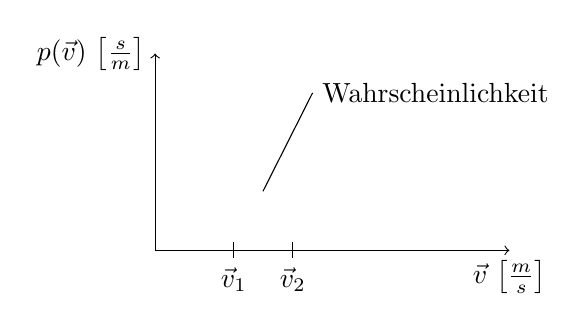
\begin{tikzpicture}[domain=0:4]
		\draw[->] (0,0) -- (4.5,0) node[below] 
			{$\vec{v}\,\left[\frac{m}{s}\right]$};
		\draw[->] (0,0) -- (0,2.5) node[left] 
			{$p(\vec{v})\,\left[\frac{s}{m}\right]$};

		\draw[color=blue, samples=200, thick] plot[id=h] 
			function{5*(x*x)*exp(-1*x*x)};

		\draw[fill=red!50, domain=1:1.75] plot[id=w] 
			function{5*(x*x)*exp(-1*x*x)} -- (1.75,0) -- (1,0) -- cycle;

		\draw[] (1,0.1) -- (1,-0.1) node[below] {$\vec{v}_1$};
		\draw[] (1.75,0.1) -- (1.75,-0.1) node[below] {$\vec{v}_2$};

		\draw[] (1.37,0.75) -- (2,2) node[right] {Wahrscheinlichkeit};
	\end{tikzpicture}
	\caption{Wahrscheinlichkeit für $P(\vec{v}_1, \vec{v}_2)$}
	\label{fig:wahrscheinlichkeit}
\end{figure}

\section{Charakteristische Geschwindigkeiten}
Wahrscheinlichste Geschwindigkeit
\[ \boxed{v_w = \sqrt{\frac{2 \cdot k_B \cdot T}{m_{kül}}} 
= \sqrt{\frac{2 \cdot R \cdot T}{m_{mol}}}} \]
Durchschnittsgeschwindigkeit
\[ \boxed{v_{av} = \langle v \rangle 
= \sqrt{\frac{8 \cdot k_B \cdot T}{\pi \cdot m_{kül}}} 
= \sqrt{\frac{8 \cdot R \cdot T}{\pi \cdot m_{mol}}}} \]
Root Mean Square Geschwindigkeit
\[ \boxed{v_{rms} = \sqrt{\langle v^2 \rangle} 
= \sqrt{\frac{3 \cdot k_B \cdot T}{m_{kül}}} 
= \sqrt{\frac{3 \cdot R \cdot T}{m_{mol}}}} \]

\begin{comment}
\section{Maxwell-Boltzmann Verteilung}
\[ \boxed{f(v) = 4 \pi \left(\frac{m_{mol}}{2 \pi \cdot R \cdot T}\right)
^{\frac{3}{2}} \cdot v^2 \cdot e^{-\left(\frac{m_{mol} \cdot v^2}
{2 \cdot R \cdot T}\right)}} \]
\[ \boxed{f(v) = 4 \pi \left(\frac{m_{kül}}{2 \pi \cdot k_B \cdot T}\right)
^{\frac{3}{2}} \cdot v^2 \cdot e^{-\left(\frac{m_{kül} \cdot v^2}
{2 \cdot k_B \cdot T}\right)}} \]
Wahrscheinlichkeit:
\[ \boxed{P(v_1, v_2) = \int\limits_{v_1}^{v_2} f(v) ~ dv} \]

\section{Charakteristische Geschwindigkeiten}
Wahrscheinlichste Geschwindigkeit
\[ \boxed{v_w = \sqrt{\frac{2 \cdot k_B \cdot T}{m_{kül}}} 
= \sqrt{\frac{2 \cdot R \cdot T}{m_{mol}}}} \]
Durchschnittsgeschwindigkeit
\[ \boxed{v_{av} = \langle v \rangle 
= \sqrt{\frac{8 \cdot k_B \cdot T}{\pi \cdot m_{kül}}} 
= \sqrt{\frac{8 \cdot R \cdot T}{\pi \cdot m_{mol}}}} \]
Root Mean Square Geschwindigkeit
\[ \boxed{v_{rms} = \sqrt{\langle v^2 \rangle} 
= \sqrt{\frac{3 \cdot k_B \cdot T}{m_{kül}}} 
= \sqrt{\frac{3 \cdot R \cdot T}{m_{mol}}}} \]
\end{comment}
